\documentclass[10pt,journal,compsoc]{IEEEtran}
\usepackage{graphics}
\graphicspath{ {Figures/} }
\usepackage{float}
\usepackage{balance}
\usepackage{times}
\usepackage{url}
\usepackage{subfigure}
\usepackage{color}
\usepackage[pdftex]{hyperref}
\usepackage{subfigure}
\usepackage{textcomp}
\usepackage{color}
\usepackage{capt-of}
\usepackage{mathtools}
\usepackage{amsmath}
\usepackage{algorithm,algorithmic}
\usepackage{multirow}
\usepackage{soul}

\usepackage{times}
% To make various LaTeX processors do the right thing with page size.


% End of preamble. Here it comes the document.

\begin{document}

\title{Asthma Pattern Identification via Continuous Diaphragm Motion Monitoring}

\author{Menghan~Liu and Ming-Chun Huang% <-this % stops a space
\IEEEcompsocitemizethanks{\IEEEcompsocthanksitem Menghan Liu is with the Department
of Electrical Engineering and Computer Science, Case Western Reserve University, Cleveland, OH 44106.
\protect\\
% note need leading \protect in front of \\ to get a newline within \thanks as
% \\ is fragile and will error, could use \hfil\break instead.
E-mail: mxl677@case.edu}% <-this % stops an unwanted space
\IEEEcompsocitemizethanks{\IEEEcompsocthanksitem
Ming-Chun Huang is with the Department
of Electrical Engineering and Computer Science, Case Western Reserve University, Cleveland, OH 44106.
\protect\\
% note need leading \protect in front of \\ to get a newline within \thanks as
% \\ is fragile and will error, could use \hfil\break instead.
E-mail: ming-chun.huang@case.edu}% <-this % stops an unwanted space
}





\IEEEtitleabstractindextext{%
\begin{abstract}
Ultrasound imaging has been widely used in bio-medical imaging diagnosis for a long history because of its merits: no radiation, high penetration depth, and real-time imaging capability. In this paper, we propose an ultrasound-based system that monitors respiratory status of asthma subjects via detecting of diaphragm movement. This system implements Chan-Vese algorithm to accurately segment diaphragm area from ultrasound image sequences and extracts 1D breathing waveform by computing mutual information (MI) between two consecutive ultrasound frames. In addition, four types of respiratory signals are identified: normal breath, fast breath, apnoea, and cough, which are related to four symptoms of asthma attack and defined as the breathing templates used for early asthma detection. In experiments, the proposed system is evaluated with a public dataset from 'Ultrasound image gallery' which contains 9 ultrasound videos and our dataset collected by 'Interson Seemore' probe which contains 5 ultrasound videos in the diaphragm area. The results show that Chan-Vese segmentation method is superior to the other three algorithms: adaptive thresholding, EM/MPM, and Fuzzy C Means (FCM), and MI is a feasible method to extract accurate respiratory signal and clear information of the phase of respiratory cycle from 2D images.

\end{abstract}

% Note that keywords are not normally used for peerreview papers.
\begin{IEEEkeywords}
Ultrasound, Image Segmentation, Respiration Signal Extraction, Asthma Pattern.
\end{IEEEkeywords}}

\maketitle


\section{introduction} \label{sec.introduction}

Asthma is a common and worldwide chronic inflammatory disease of the airway. It is characterized by variable and recurring symptoms, reversible airflow obstruction, and bronchospasm. Its common symptoms include recurring wheezing, coughing, chest tightness, fast breathing, and shortness of breath. The occurrence of asthma has increased significantly since the 1970s. In 2011, 235 million people have been diagnosed with asthma and asthma attack caused 250,000 deaths globally~\cite{Varsha:2014}. This number increased to 334 million in 2014~\cite{Asthma:2014}. Meanwhile, in the United States, asthma prevalence increased from 7.3 \% in 2001 to 8.4\% in 2010. 25.7 million persons had asthma in 2010, that means one of 12 people had asthma. Among these asthma patients, more than half of them has experienced an asthma attack. What's worse, asthma results in a high cost for individuals and the nation. In the United States, every person with asthma spent 3,300 dollars each year from 2002-2007 in medical expenses and the overall nation-wide expense is about 56 billions for medical costs, lost school, work days, and early deaths in 2007~\cite{Vitalsigns:2011}.

However, many asthma attacks could be  prevented. For example, if patients know how to identify and avoid asthma triggers, then they could try to be away from those triggers. Besides that, monitoring breath is also very important, which can recognize warning symptoms of an impending asthma attack, such as slight coughing, wheezing, and shortness of breath. Sometimes, lung function decreases before any symptoms are noticed. Those subjects who have airway obstruction for a long time are less likely to be aware of dyspnoea than subjects with acute onset of airway obstruction. In another word, subjects are more likely to be aware of the poor function of lung with hypoxia during an acute exacerbation, predisposing to severe, and life threatening attacks. Therefore, monitoring lung function and condition are very important for looking after asthma patients, early detecting exacerbations, and controlling asthma day-to-day. Currently, asthma patients have to take asthma examine with an interval of at least 2 to 3 months between visits. However, it is vulnerable for recalling bias as a result of retrospective assessment of symptoms when physicians evaluate asthma control during clinical visits. Wireless/portable ultrasound  becomes a desirable approach for asthma control because it can continuously monitor lung function and asthma symptoms in home environment. It is more efficient than taking asthma examine periodically~\cite{Dillys:2014}. Therefore, it is crucial to investigate a computational method for evaluating asthma in home environment.

Nowadays, proposed methods for monitoring asthma are usually based on lung volume, gas sensing, and imaging. The first two types of technology cannot provide continuous and real-time information of user's breathing. However, ultrasound devices instead can be used in portable forms~\cite{huang2013high}\cite{wygant2008integration}\cite{kurtz2013usefulness} and  have the ability to collect real-time images of the organs and their movement information~\cite{hwang2012robust}\cite{Christian:2011}. Therefore, ultrasound could be applied to detect respiratory signal via diaphragm movement monitoring~\cite{Daniel:2008}\cite{Xu:2006}. There are still some difficulties in implementing ultrasound images of diaphragm movement. First, ultrasound images have some properties: gray-scale, attenuation, speckle, blurred boundaries, and low contrast between region of interest and background, which makes proper segmentation difficult. In addition, many areas have the same gray value as the detected diaphragm area, which make the segmentation task of crescent diaphragm area more complicated. Therefore, an appropriate segmentation method needs to deal with these problems. Lichtenstein~\cite{Daniel:2008} and Xu~\cite{Xu:2006} applied simple threshold-based segmentation algorithms, but they cannot ensure the accuracy of segmentation in low-quality ultrasound images. To solve the problems mentioned above, we propose a system to extract respiratory signals from ultrasound videos collected by a portable ultrasound device. Implemented Chan-Vese algorithm of the developed system is robust for locating diaphragm areas in low-quality ultrasound image sequences. Another contribution of this paper is defining four typical templates of asthma respiratory patterns. Respiratory symptoms accompanying with asthma attack occurrence include frequent cough, breathing faster than normal, shortness of breath, decreasing in a peak expiratory flow, and upper respiratory inflection~\cite{ACAAI:2013}\cite{National:2013}. Catterall et al.~\cite{catterall1982irregular} discussed four respiratory patterns of asthma subject detected by oronasal air flow. However, they did not build a relation between respiratory patterns of irregular symptoms and the occurrence of asthma attack. In this paper, we identify one normal breathing pattern and three irregular patterns related to three symptoms of asthma attack: frequent cough, breathing faster than normal, and shortness of breath. These patterns are extracted from ultrasound image sequences and defined as breathing templates. By splitting respiratory signals and comparing them with the stored templates, symptoms of asthma attack can be detected. The benefit of breathing signal extraction from 2D ultrasound is that when irregular breathing signal is detected, doctors/researchers can retrieve ultrasound images back to figure out how organ moves at that period, thus they will obtain more information for asthmatic analysis.

The remainder of this paper is structured as follows. In Section 2, background of asthma and ultrasound is introduced. Section 3 provides some relevant works in the area of asthma detection. Then the proposed ultrasound-based system and algorithm are introduced in Section 4. In Section 5, the system is evaluated with experiments and the four breathing templates are explained. The evaluation includes a comparison of four segmentation methods, accuracy of computed respiratory rate, and a correspondence between the phase of respiratory cycle and the diaphragm location.

\section{Preliminary} \label{sec.preliminary}

\begin{figure}[h!]
\centering
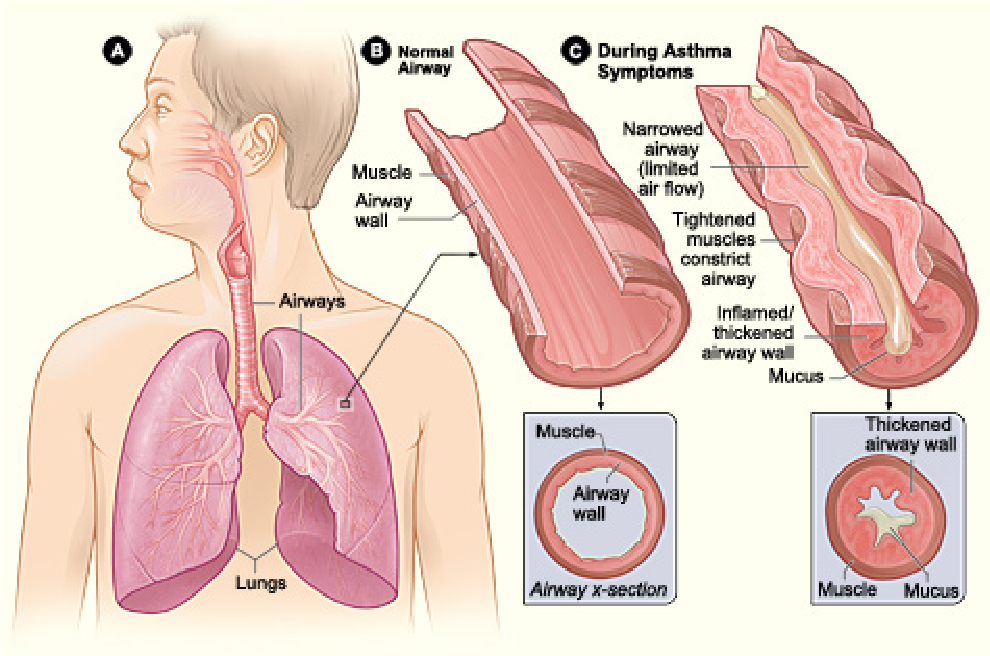
\includegraphics[width=0.36\textwidth]{Aasthma.pdf}
\caption{Concept diagram of asthma formation~\cite{NH}}
\label{fig.Asthma}
\end{figure}
Figure~\ref{fig.Asthma} shows how the airway narrows when asthma attack occurs. Airways are tubes that carry air into and out of our lungs. People who have asthma attack experience usually have inflamed airways. When the airways respond to triggers, the muscles around the airways will tighten. In addition, mucus is a sticky, thick liquid that can further make the airways narrow and narrowed airways allow less air to flow into lungs. As a result, asthma symptoms may occur, such as recurring periods of wheezing (a whistling sound when you breathe), chest tightness, shortness of breath, and coughing.

The breathing activity is performed primarily by the diaphragm, a large muscle that separates the thoracic cavity from the abdominal cavity. During inspiration (breathing in), diaphragm contracts, draws downward, and creates a vacuum in thoracic cavity. This vacuum inflates lungs by drawing air into body through the trachea or windpipe. During normal expiration (breathing out), the diaphragm relaxes and allows air to flow out as the lungs deflate, similar to the way that an inflated balloon deflates when releases. When people have asthma attack, their respiratory pattern changes and the movement pattern of diaphragm also changes.

Ultrasound is a non-invasive and real-time tool used for imaging soft tissues. Medical ultrasound is based on the use of high frequency sound to aid in diagnosis and treatment of patients. Usually, ultrasound frequencies range from 2 to 15 MHz approximately. Ultrasound waves (pulses of sound) are emitted from a transducer, propagate through different tissues, and return to the transducer as reflected echoes. Ultrasound is conducted with different speeds in a various of body tissues. Some tissues absorb sound waves while others reflect them. The density of the tissues corresponds to the speed at which the echoes return. There are different ways to visualize the obtained ultrasound information, which are called ultrasound modalities. The most common modes are A-mode, B-mode, and M-mode. The 'A' in A-mode stands for Amplitude. Information of the reflected signal in a single ultrasound beam is continually displayed. Distance from the transducer and signal intensity are shown by position and amplitude as a line on an oscilloscope. This mode is mainly used for historical interest. The 'B' in B-mode stands for Brightness. B-mode information can form a sector in a plane of the body, shown as pixel intensity on a monitor. In B-mode ultrasound image, fluid is black, tissue is gray, and bone is white. The denser the tissue is, the brighter white it appears. The brightest white is bone. B-mode often generates 2D image, which  is the most important modality for anatomic assessment and orientation in the body. The 'M' in M-mode stands for Motion. This represents movement of ROI over time. The M-mode has good temporal resolution, so that it is useful in detecting and recording rapid movements. In this paper, the goal is to locate the diaphragm region in ultrasound image. For this reason, we choose the B-mode to collect data as Youngkyoo suggested~\cite{hwang2012robust}.



\section{related work} \label{sec.relatedwork}
Scientists proposed many methods based on lung volume, gas sensing, and imaging~\cite{Lorenzo:2013}.
In terms of lung volume methods, peak expiratory flow (PEF) is the most commonly used parameter for monitoring lung function of asthma patients. It is very popular in primary care because it can be measured easily by simple, cheap and portable devices. Forced Expiratory Volume in 1 Second (FEV$_1$) is also a widely used standard for  measuring airflow caliber. However, methods measuring these two parameters have some common limitations: lack of compliance, possible falsification of results, and long recording periods~\cite{Moscato:1995}.
Gas sensing method is another sensing modality to detect asthma by monitoring Nitric oxide (NO) and CO$_2$. NO gas level will increase when asthma attack occurs~\cite{Kharitonov:1994}. The CO$_2$ output patterns between healthy and asthma-suffering patients are different~\cite{You:1994}.
Furthermore, with the development of sophisticated imaging techniques, image of lung in asthma patients has evolved dramatically over decades, such as positron emission tomography (PET), magnetic resonance imaging (MRI), single photon emission computed tomography (SPECT), and ultrasound (US). These techniques provide different approaches to visualize gross anatomic abnormalities, regional lung mechanics, and airway anatomy. They are also very useful for understanding the different functions between the lungs of healthy subjects versus asthma patients~\cite{Mario:2011}.
Compared with these oneshot images methods, ultrasound method can capture image sequences of moving organs and tissues, which enables users perform real-time analysis of respiration via ultrasound imaging technology. Better portability and no radiation are another two advantages of ultrasound sensing modality. Thus, it will be safer for long-time monitoring and can be used with special group of people, such as pregnant women and children.
\begin{figure*}[htb]
\centering
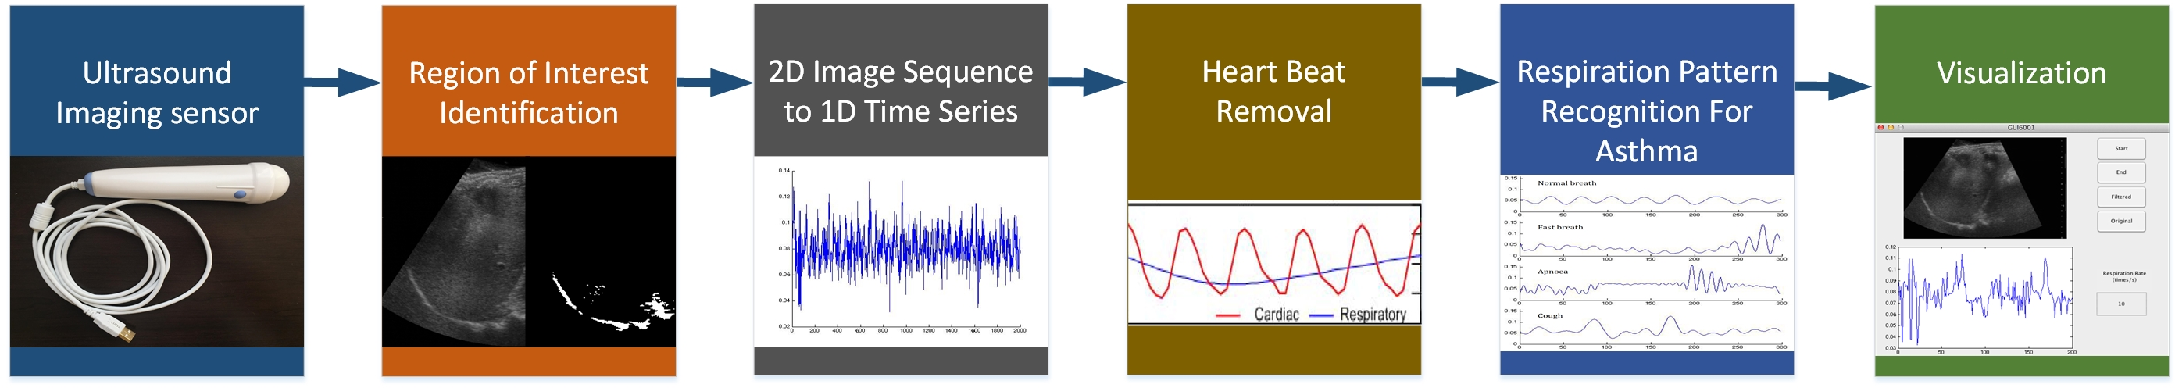
\includegraphics[width=1\textwidth]{Framework.pdf}
\caption{Overview of the ultrasonography processing procedures}
\label{fig.System}
\end{figure*}

There are many proposed approaches to detect respiratory motions based on ultrasound devices. Bruin et al.~\cite{Bruin:1997} found that asthma patients had thinker $D_iT_{relax}$, diaphragm thickness during relaxation. So they measured $D_iT_{relax}$ from B-mode ultrasound images to detect asthma patterns.
Researchers also could infer respiration pattern by quantifying the movements of a kidney, because kidney moves along with breathing~\cite{Laurent:1994}. According to research of Wachinger et al.~\cite{Christian:2011}, the neighborhood relationship of organs is related with breathing cycle. They measured respiration by investigating 2D ultrasound images of liver and kidney. This method has the advantage that it is fully automatic and does not require a training phase or prior information about underlying anatomy, nor the interaction of user.
Tuathan et al.~\cite{Tuathan:2014} proposed a 2D normalized cross-correlation (NCC) based algorithm to estimate movement of a liver in 2D ultrasound images. But, due to the blur boundaries of kidney and liver in low contrast ultrasound image, the performance of  monitoring still requires further improvement.
In 2006, Xu et al.~\cite{Xu:2006} proposed a novel respiratory detection method based on diaphragm motion using a 2D ultrasound unit. Because white diaphragm region in ultrasound image is outstanding among  dark regions of organs, their method could easily extract respiratory signal from an automated analysis of the internal diaphragm movement during breathing. They selected the region of interest (ROI) and computed the mutual information (MI) and correlation coefficient (CCs) between reference ultrasound frame and all other frames. From their experiments, they discovered that MI and CC values produced a 1D signal corresponding to the respiratory cycle in both phase and magnitude.
In 2012, Hwang et al.~\cite{Youngkyoo:2012} proposed a system that placed feature windows on ROI of each ultrasound image and calculated organ's displacement through feature windows. Their proposed method can robustly extract respiratory motion signal with regardless of reference frame, because this method computed actual organ's displacement instead of similarity measurement like MI or CC. This method could provide clear information of the phase of respiratory cycle such as inspiration and expiration. The drawback of Hwang's approach is that adaptive thresholding algorithm implemented in his paper cannot detect diaphragm region robustly.

In this paper, we propose a system to perform analysis of respiration, which implements Chan-Vese algorithm to segment the diaphragm area from ultrasound image sequence accurately and identifies respiratory signals corresponding to diaphragm activities. To reduce the interference of cardiac motion, this system performs low-pass filter to purify time-series signals. Furthermore, in order to detect asthma attack by monitoring irregular breathing symptoms, we identify one normal breathing template and three irregular templates related to the three symptoms of asthma attack: frequent cough, breathing faster than normal, and shortness of breath. By comparing with these four templates, the proposed system can detect irregular respiratory patterns and notify asthma attack occurrence. 
\section{System Overview} \label{sec.system}

\begin{figure*}[htb]
\centering
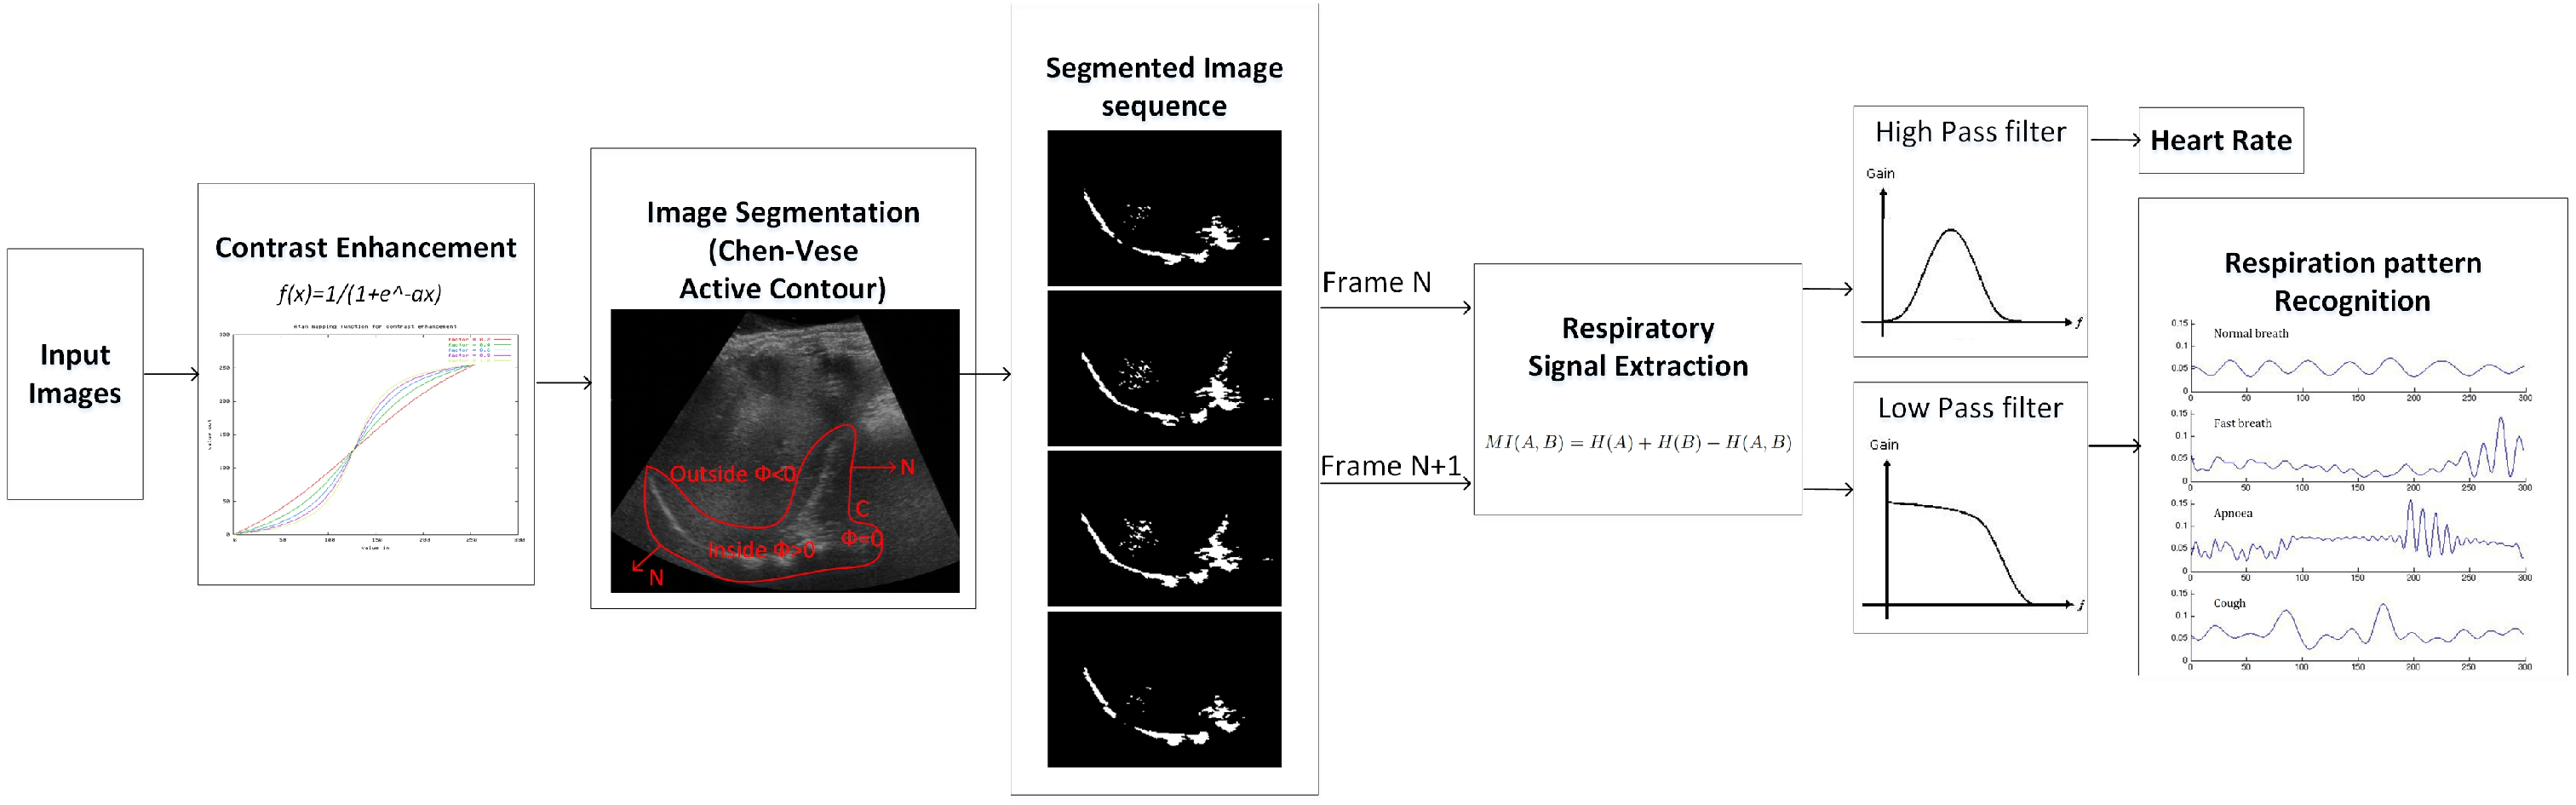
\includegraphics[width=1\textwidth]{flowchart.pdf}
\caption{Image analysis flowchart}
\label{fig.flow}
\end{figure*}
In this section, the system design of asthma pattern identification is discussed. It consists of six parts: a USB ultrasound imaging probe, ROI Identification, 2D Image Sequence to 1D Time Series, heartbeat removal, respiratory pattern recognition for asthma, and visualization, as shown in Figure~\ref{fig.System}.

First of all, ultrasound probe collects ultrasound image sequences around liver and diaphragm locations. Then these images are transmitted via USB to a computer. In this paper, the goal is to monitor the movement of diaphragm to extract respiratory signal, so system identifies and segments the diaphragm area in the image sequence, and then computes 1D time-series signal drawn by mutual information (MI) which reflects relation among consecutive ultrasound image sequence. The original 1D waveform contains respiratory signal and unwanted interference, such as cardiac signal. Therefore, a low-pass filter is used to get rid of interference and preserve low respiratory frequency. Next, the computed 1D signal is compared to four templates: normal breath, fast breath, apnoea, and coughing. In the end, ultrasound video, original signal, purified signal, and respiration rate are displayed on a designed Matlab user interface.
\subsection{Ultrasound Sensor System}
In experiments, an ultrasound probe from Interson company is used, which is a USB ultrasound probe system. Detailed technical specifications are listed in Table~\ref{tab.Spec}.
\begin{table}
\newcommand{\tabincell}[2]{\begin{tabular}{@{}#1@{}}#2\end{tabular}}
 \centering
 \begin{tabular}{|c|c|}\hline
Depth Range & \tabincell{c}{2-15 cm } \\\hline
Pulse Frequency & \tabincell{c}{3.5-5MHz} \\\hline
Frame Rate & \tabincell{c}{12 fps } \\\hline
Scan Angle & \tabincell{c}{60 degrees } \\\hline
Image Format & \tabincell{c}{Jpeg } \\\hline
Image Size & \tabincell{c}{$1024\times600$} \\\hline
Gray Scale & \tabincell{c}{256 shades } \\\hline
Scanning Mode & \tabincell{c}{B-mode } \\\hline
\end{tabular}
\vspace{0.3 cm}
\caption{Technical specifications of Interson ultrasound imaging probe}
\label{tab.Spec}
\end{table}
This transducer converts ultrasound waves to electrical signal and perform B-mode scanning to generate ultrasound images. Images are transmitted to a computer via USB. Direct streaming of B-mode ultrasound images is used over this system. As the ultrasound waves penetrate body tissues of different acoustic impedances, some are reflected back to the transducer (echo signals) and some continue to penetrate deeper. The echo signals returned from many sequential coplanar pulses are processed and combined to generate an image. The pulse frequency of this probe is 3.5 to 5 MHz and the largest scan depth is about 15 cm. It can detect the movement of organs and tissues in our body, such as a liver, kidney, lung, and diaphragm. The sample frequency is 12 frames per second which is much higher than the breathing frequency. The collected data are high quality JPEG images with 256 shades of gray scale. Image size is $1024\times600$ pixels.

\subsection{Image Analysis}
Collected images are processed to extract respiratory signals, and use these signals to compute the breathing rate and evaluate the respiratory pattern. Image analysis contains segmentation of ROI, 1D respiratory signal extraction with MI method, and filter. Finally, the purified respiratory signal is compared with the stored templates to classify pattern of asthma. The image analysis flowchart is shown in Figure~\ref{fig.flow}.

\textbf{4.2.1 Chan-Vese active contour}

 This system implements the Chan-Vese active contour algorithm~\cite{Chan:2001} to find ROI. The basic idea of this model is that starting with a curve around the objects, the curve extends or shrinks toward its interior normal, and stops when touch the boundary of the objects. Given an image $u_0$, the goal is to look for the best approximation $u$ of $u_0$ by minimizing an energy function $F(c_1, c_2, C)$. $u$ is the segmented result and it takes two values:
\begin{equation}
u=
\begin{cases}
average(u_0),  &\mbox{ inside C}\\
average(u_0),  &\mbox{ outside C}\\
\end{cases}
\end{equation}

Notations are illustrated in Figure~\ref{fig.curve}. The energy function $F(c_1, c_2, C)$ is defined by\\
\begin{align*}
F(c_1, c_2, C) =&\mu \int_{\Omega}\delta(\phi (x, y))|\bigtriangledown\phi(x, y)|{d}x{d}y\\
                    &+\nu \int_{\Omega}H(\phi (x, y)){d}x{d}y\\
                    &+\lambda _1\int_{\Omega}|u_0(x, y)-c_1|^2H(\phi (x, y)){d}x {d}y\\
                    &+\lambda _2\int_{\Omega}\mid u_0(x, y)-c_2\mid ^2\\
                    &(1-H(\phi (x, y))){d}x{d}y\\
\end{align*}
where $C$ is an arbitrary variable curve, and constants $c_1$, $c_2$, depending on C, are averages of $u_0$ inside $C$ and respectively outside $C$. $\mu \geq0$, $\nu \geq0$, $\lambda _1$, $\lambda _>0$ are fixed parameters and function $H$ is the Heaviside function, defined by:
\begin{equation}
H(z)=
\begin{cases}
1,  &\mbox{ if $z \geq 0$}\\
0,  &\mbox{ if $z \leq 0$}\\
\end{cases}
\end{equation}
In this equation, the first item is the length of curve and the second item is the area of the region inside. They are the regularizing items.
Primary steps of the algorithm are shown in Algorithm 1.
\begin{algorithm}
\caption{Chan-Vese active contour algorithm}
\begin{algorithmic}
%\STATE
\STATE /* Initialization */
\STATE Step 1: $\phi^0\leftarrow\phi _0, n\leftarrow0$.
%\STATE
\STATE /* Iteration */
\STATE Step 2: Compute $c_1(\phi^n)$ and $c_2(\phi^n)$.
\STATE Step 3: Solve the PDE in $\phi$ to obtain $\phi^n+1$.
\STATE Step 4: Reinitialize $\phi$ locally to the signed distance function to the curve (this step is optional).
\STATE Step 5: If the solution is stationary, stop,
\STATE \qquad \qquad otherwise go to Step 2.
\end{algorithmic}
\end{algorithm}

\textbf{4.2.2 Breathing signal extraction}
Mutual information (MI) is computed as the 1D signal. MI measures statistical dependence of two images and is defined by
\begin{align*}
MI(A,B) &=H(A)+H(B)-H(A, B)\\
            &=\sum\limits_{ab} p(a, b)log\dfrac{p(a, b)}{p(a)p(b)}\\
\end{align*}
Here, $A$ and $B$ are ROI from two consecutive image frames. $H(A)$, $H(B)$, and $H(A, B)$ are the entropies of $A$ and $B$, and their joint entropy respectively. $p(a, b)$, $p(a)$ and $p(b)$ are the joint probability distribution of $a$ and $b$, and their individual probability distributions, where $a$ and $b$ are the pixel values in $A$ and $B$.
An image at the end of inspiration is selected as a reference image. MI between this frame and all other segmented image frames were computed. Large MI value occurs when diaphragm is close to the reference frame, i.e. the end of inspirations. On the contrary, small MI value occurs when the diaphragm motion is far away from the reference. Thus 1D signal's magnitude and phrase are related to respiration.

\begin{figure}[h!]
\centering
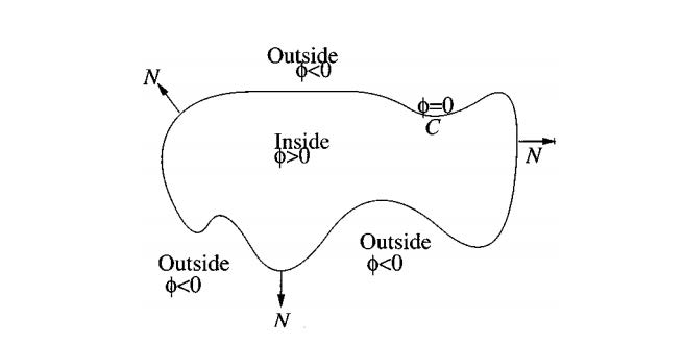
\includegraphics[width=0.36\textwidth]{curve.pdf}
\caption{Curve \textbf{$C=(x, y): \phi(x, y)=$} propagation in normal direction}
\label{fig.curve}
\end{figure}


\textbf{4.2.3 Heartbeat removal}
During ultrasound images recording, the two most common sources of diaphragm motion are respiratory and cardiac motions. For the reason that asthma attack detection is only based on respiration, the cardiac signals are interference. According to Hari et al.~\cite{Hari:2009}, the cardiac signal is approximately centered at 1Hz. The time of one respiration cycle is about three seconds recorded by chronograph and the frequency of respiratory signal is around 0.3 Hz. Then the cardiac signal the respiratory signal are separated with a low pass filter.

\textbf{4.2.4 Asthma pattern templates creation}
Before asthma attack, patients usually feel some symptoms, like fast breathing, short of breath, and coughing. These symptoms will induce the change of the respiratory pattern. In this paper, four typical respiratory waveforms are used as templates, one regular template and three irregular templates: normal breath, fast breath, apnoea and cough. Fast breath is due to short of breath. Subject needs to increase breathing frequency to overcome the difficult breathing caused by narrow airways. If airways are more and more narrow, subject has the potential to get apnoea and stop breathing. Coughing also changes the breathing status. Building templates of irregular patterns is very useful for detecting asthma attack. Respiratory signal is partitioned into time segments and compare each segment with templates. Then it is efficient to identify which irregular activities happens and their occurring order.

\subsection{Visualization}
For convenience, system has a Matlab user interface to display the respiratory signal and respiration rate, as shown in Figure~\ref{fig.GUI}. Designed system could detect subject's real-time respiration status based on the movement of the diagram. The user interface contains three parts, the left part displays the ultrasound video obtained by the probe and the 1D respiratory signal. The 'operation' panel consists of four push buttons: Start, End, Filtered, and Original. When 'Filtered' button is clicked, it shows the purified respiratory signals without heartbeat interference. When click 'Original' button, it shows the mixture of heartbeats and breathing signals. 'Respiration rate' panel shows the number of respiration cycles per minute and it renews every minute.

\begin{figure}[h!]
\centering
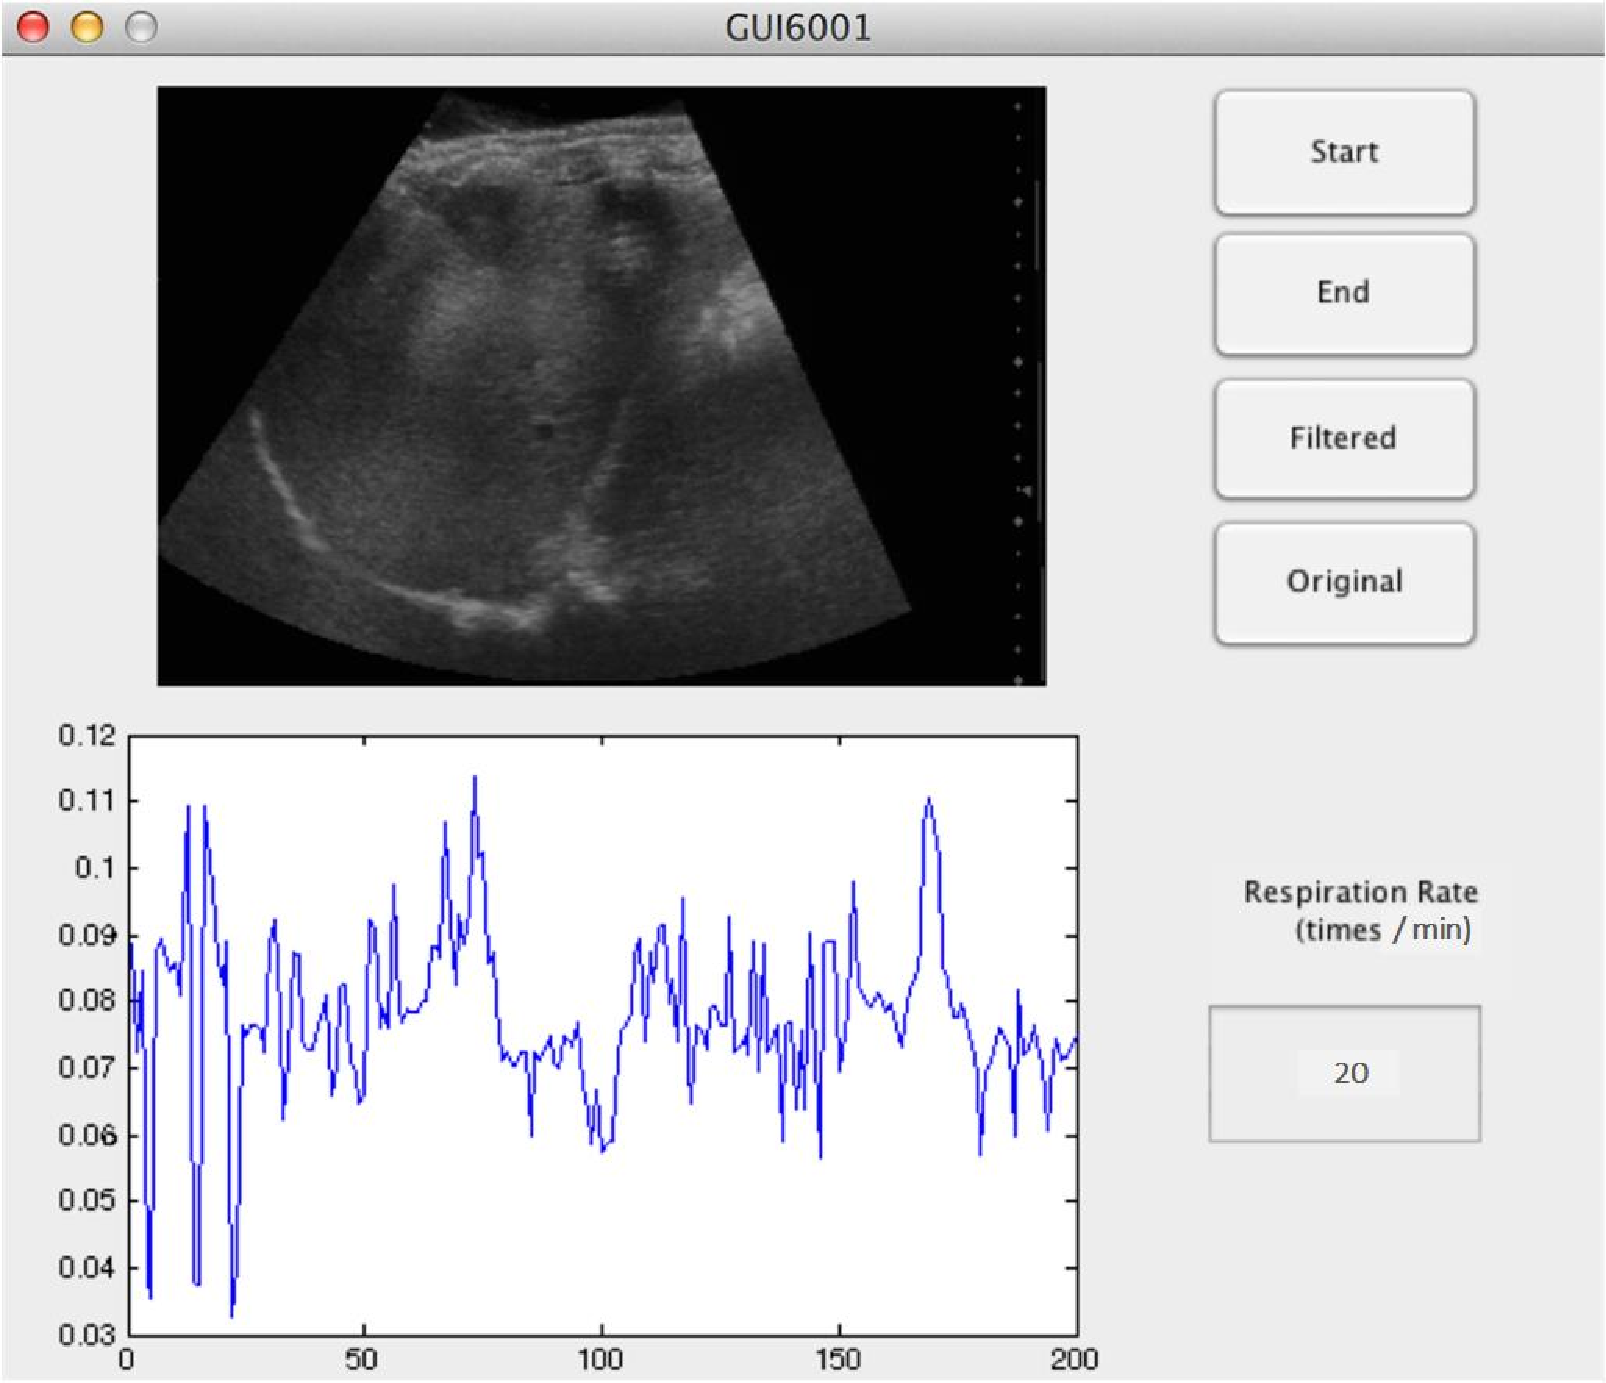
\includegraphics[width=0.36\textwidth]{MatlaGUI.pdf}
\caption{User interface design}
\label{fig.GUI}
\end{figure}

\section{Experiment} \label{sec.experiment}
\subsection{Experiment design}
To evaluate the designed system, a public dataset and our own dataset are both used in conducting experiments.
The public dataset is from Petrusca et al.~\cite{database}, which can be downloaded from "https://www.vision.ee.ethz.ch/datasets/index.en.html". It contains videos of diaphragm movement from 9 volunteers. Each volunteer performed regular breath for five and half minutes. The ultrasound device is Antares (Siemens Medical Solutions). Sample rate is from 15 to 25 frames per second and center frequency of ultrasound is about 2 MHz. This dataset is used for evaluating the performance of image segmentation and computed respiration rate. More details about the dataset are in Table~\ref{tab2.Spec}. 'V01', 'V02', ..., 'V09' are the numbers of volunteers.

\begin{table}
\newcommand{\tabincell}[2]{\begin{tabular}{@{}#1@{}}#2\end{tabular}}
 \centering
 \begin{tabular}{|c|c|c|c|c|}\hline
 Number & \tabincell{c}{Spatial \\ Resolution} & \tabincell{c}{Sample \\ rate (fps)} & \tabincell{c}{Center \\frequency\\(MHz)}& \tabincell{c}{Data \\size (GB)}\\\hline
V01 & \tabincell{c}{$640\times480$ } & \tabincell{c}{25} & \tabincell{c}{2.22} & \tabincell{c}{1.92}\\\hline
V02 & \tabincell{c}{$712\times480$} & \tabincell{c}{16} & \tabincell{c}{2.00} & \tabincell{c}{1.79} \\\hline
V03 & \tabincell{c}{$712\times480$} & \tabincell{c}{17} & \tabincell{c}{1.82} & \tabincell{c}{1.87} \\\hline
V04 & \tabincell{c}{$720\times540$} & \tabincell{c}{15} & \tabincell{c}{2.22} & \tabincell{c}{1.91} \\\hline
V05 & \tabincell{c}{$720\times540$} & \tabincell{c}{15} & \tabincell{c}{2.22} & \tabincell{c}{1.87} \\\hline
V06 & \tabincell{c}{$720\times540$} & \tabincell{c}{17} & \tabincell{c}{1.82} & \tabincell{c}{1.80} \\\hline
V07 & \tabincell{c}{$500\times480$} & \tabincell{c}{14} & \tabincell{c}{2.22} & \tabincell{c}{1.10} \\\hline
V08 & \tabincell{c}{$700\times480$} & \tabincell{c}{17} & \tabincell{c}{1.82} & \tabincell{c}{1.87} \\\hline
V09 & \tabincell{c}{$700\times480$} & \tabincell{c}{16} & \tabincell{c}{1.82} & \tabincell{c}{1.64} \\\hline
\end{tabular}
\vspace{0.3 cm}
\caption{Information of the public dataset}
\label{tab2.Spec}
\end{table}

To collect real dataset, volunteers are examined in a supine position and their diaphragm is imaged with a USB ultrasound probe (Interson Seemore) in B-mode. The probe is adjusted to 5 MHz and placed inferior of the rib cage with the fan direction aligned approximately in parallel to the lowest rib. Five volunteers are asked to breathe normally for 5 minutes and the ultrasound image sequences are collected as normal breathing dataset, named as 'Real01', 'Real02',...., 'Real05'. They are used for verifying the accuracy of the segmentation algorithms. At the same time, we record the number of breathing cycles as ground truth. Volunteers also perform coughing, quick breath, and holding breath to simulate three irregular breathing activities: coughing, fast breath, and short of breath.

\subsection{Experiment results and discussion}
The collected ultrasound videos are decomposed into individual frames for further analysis. The predominant motion is a two-dimensional profile of the diaphragm which follows the breathing cycle of the volunteers. One frame of 'volunteer02' video and its corresponding enhanced result are shown in Figure~\ref{fig.adjust}. In the following explanation, voluteer02's dataset will be used as example.
\begin{figure}[h!]
\centering
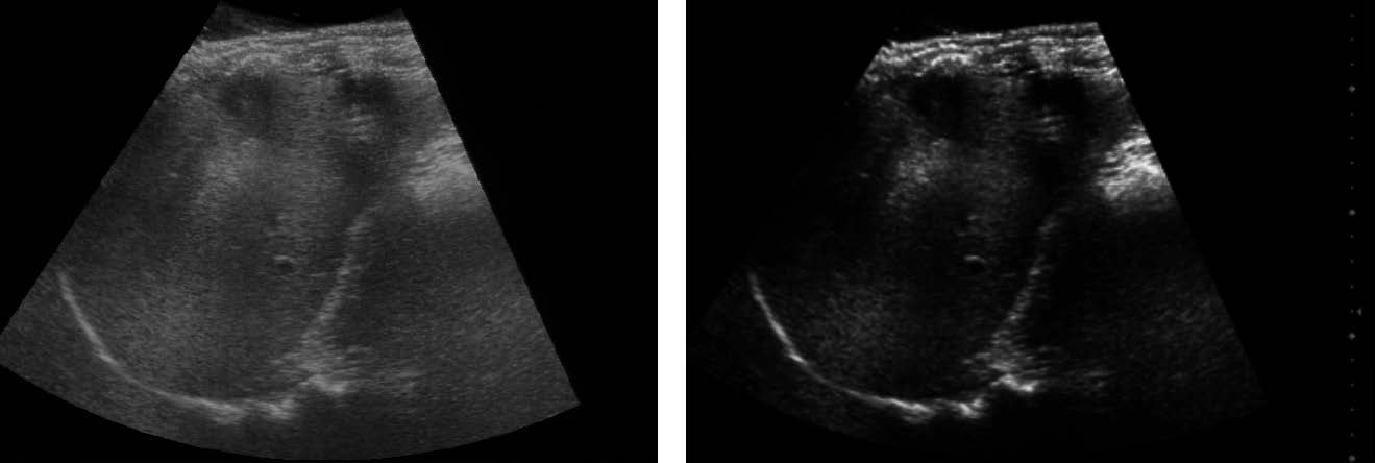
\includegraphics[width=0.36\textwidth]{adjust.pdf}
\caption{Original low contrast (left); Adjusted high contrast (right)}
\label{fig.adjust}
\end{figure}
Moreover, another problem is that the high resolution of original image results in tremendous computational time.  Downsampling images on the premise that it does not affect the quality of the segmentation is very efficient for time reduction. The segmentation result is a binary image, as shown in Figure~\ref{fig.segment}(a). The white arc is the diaphragm and the black part is other tissues and organs. Compared with the original image, shape and location of segmented areas are matched with expectation. There are some small spots above the arc of diaphragm which are the tissues of the liver. When the contour shrinks or extends around diaphragm, liver tissues are also segmented out, because it is very close to the diaphragm, lighter than background, and also in our rectangular seed. The contraction and relaxation of diaphragm force the liver to move. Movement of spots and diaphragm are in the same phase, and these spots does not affect the 1D respiration signal. In order to verify segmentation accuracy of Chan-Vese, we also do segmentation with other three algorithms as comparison: Adaptive thresholding~\cite{singh2012new}, EM/MPM algorithm~\cite{yang2012performance} and Fuzzy c-means (FCM)~\cite{bezdek1984fcm}. Results are in Figure~\ref{fig.segment}(b)-(d). These three algorithms segment out diaphragm as well as the upper white area which has the similar gray value as diaphragm area. EM/MPM result is worse. The extracted diaphragm by EM/MPN is wider than real one. Compared with these three algorithms, Chan-Vese has the advantage that it can exclude the light areas and extract the diaphragm area only. Therefore, performance of Chan-Vese in our dataset is superior.
\begin{figure}[h!]
\centering
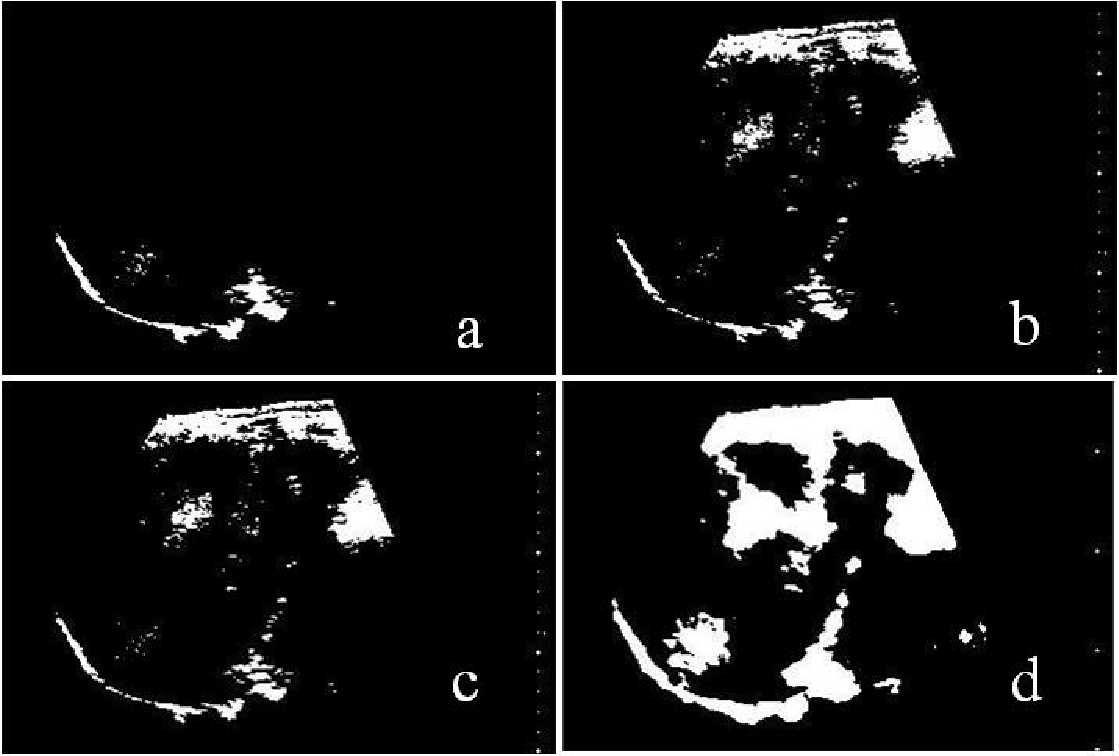
\includegraphics[width=0.36\textwidth]{CompareResult.pdf}
\caption{Comparison of Results. (a) is the segmentation by Chan-Vese algorithm; (b) is the segmentation by Adaptive Thresholding algorithm; (c) is the segmentation by Fuzzy c means algorithm; (d) is the segmentation by EM/MPM algorithm.}
\label{fig.segment}
\end{figure}

The computed MI values of consecutive images are shown in Figure~\ref{fig.orignalMI}. Because the limitation of paper's width, we only plot the first 2000 frames of voluteer02's ultrasound video. Because of the interference, such as heartbeats, we cannot straightforwardly identify clear cycles of respiration which includes peaks and valleys from original MI waveform. Therefore, we perform Fast Fourier Transform (FFT) to see frequency distribution, as shown in Figure~\ref{fig.fft}.
\begin{figure}[h!]
\centering
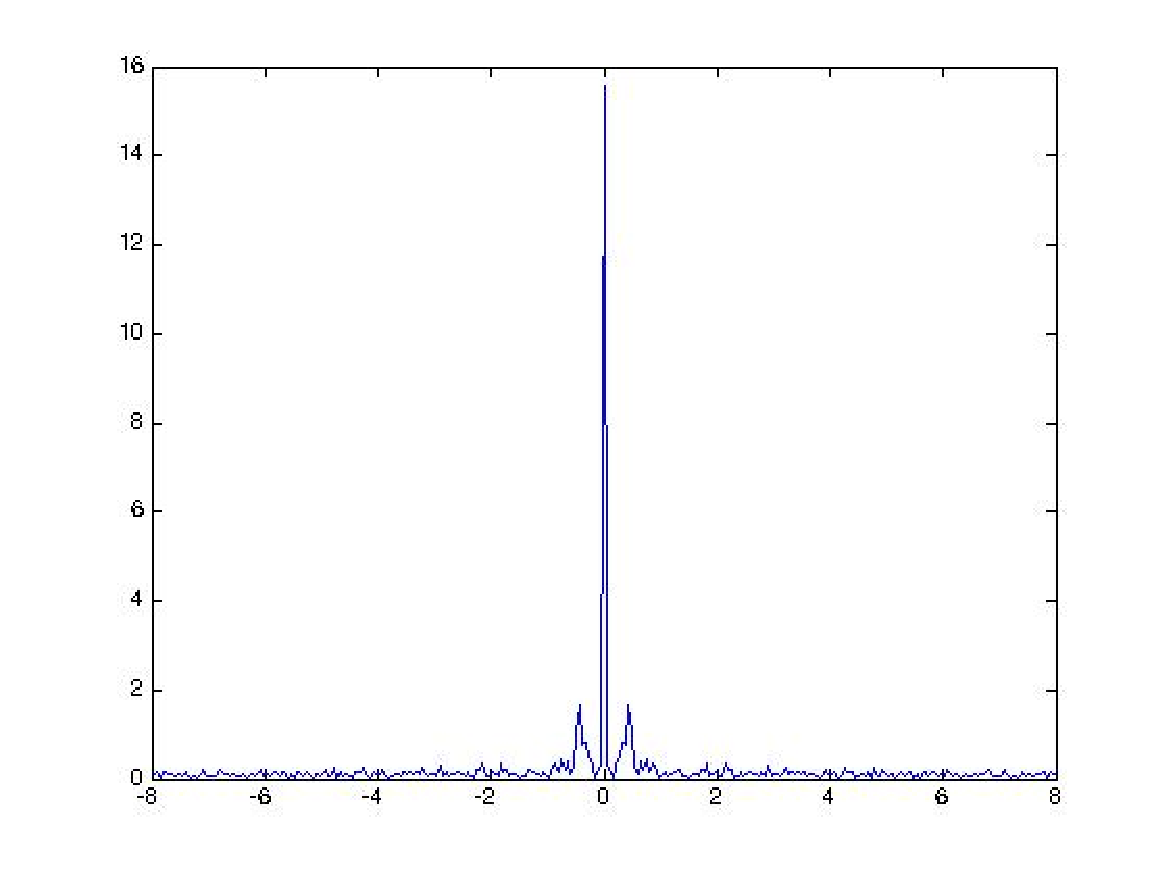
\includegraphics[width=0.36\textwidth]{normalfft.pdf}
\caption{Fast Fourier Transform of the original MI waveform}
\label{fig.fft}
\end{figure}
The respiration frequency is lower than heartbeat and it is usually less than 1Hz. In Figure~\ref{fig.fft}, FFT shows that most energy concentrates between $[-0.4 Hz, 0.4 Hz]$. A low-pass filter is designed with a threshold at 0.4 Hz to filter out noises. Then a clear respiratory signal is obtained, as shown in Figure~\ref{fig.filteredMI}. There are 38 peaks and 38 valleys in the 2000 frames. Respiration rate is 18.2 times/minute. To verify the computed result, we record the number of respiration cycles in the volunteer's video. Figure~\ref{fig.breathcycle} shows the diaphragm profile at a various of breathing phases for a typical cycle. There are 38 such cycles in this video clip and one cycle is approximately 3s, which corresponds to $3\times Sample Rate$ frames in the video file. Computational results and the corresponding ground truth are listed in Table~\ref{tab3.results}. By comparison, the computational results are very close to ground truth.

\begin{figure}[h!]
\centering
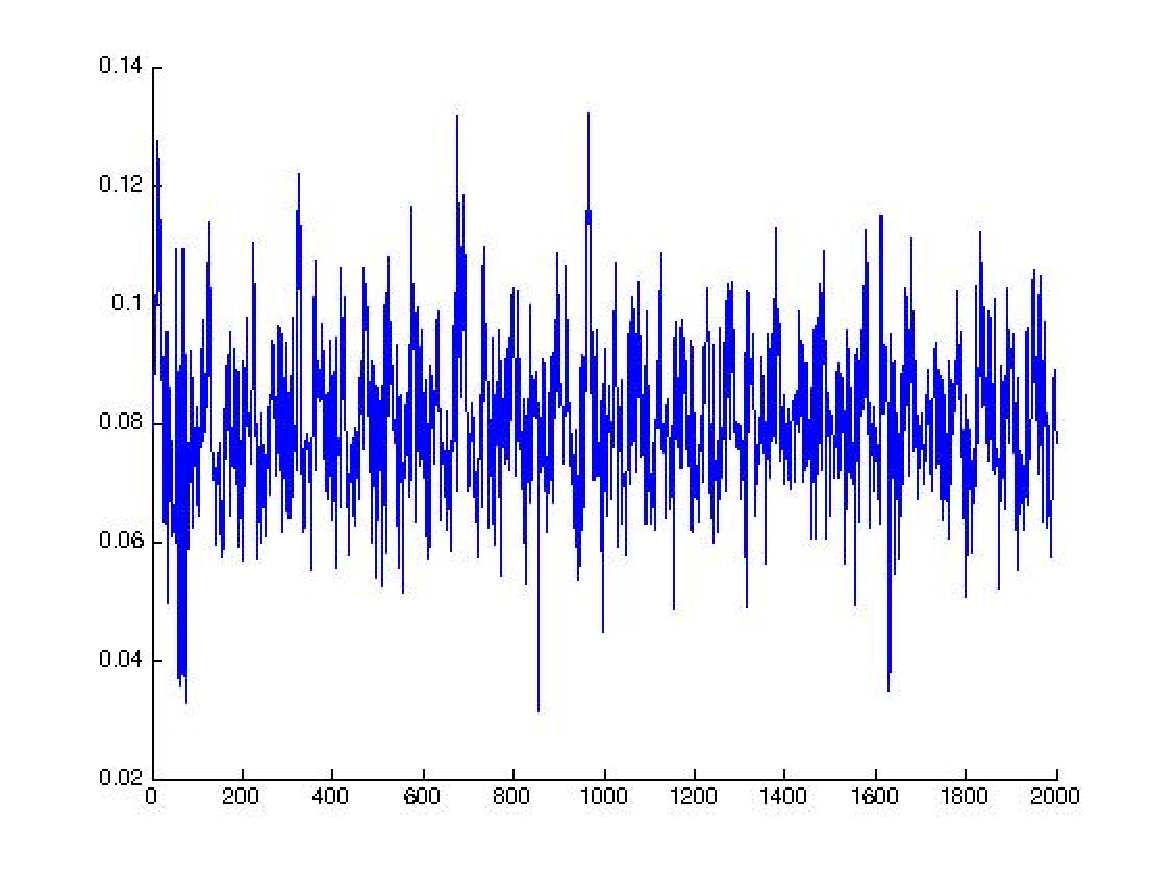
\includegraphics[width=0.36\textwidth]{orignalMI.pdf}
\caption{Noisy 1D MI signal}
\label{fig.orignalMI}
\end{figure}

\begin{figure}[h!]
\centering
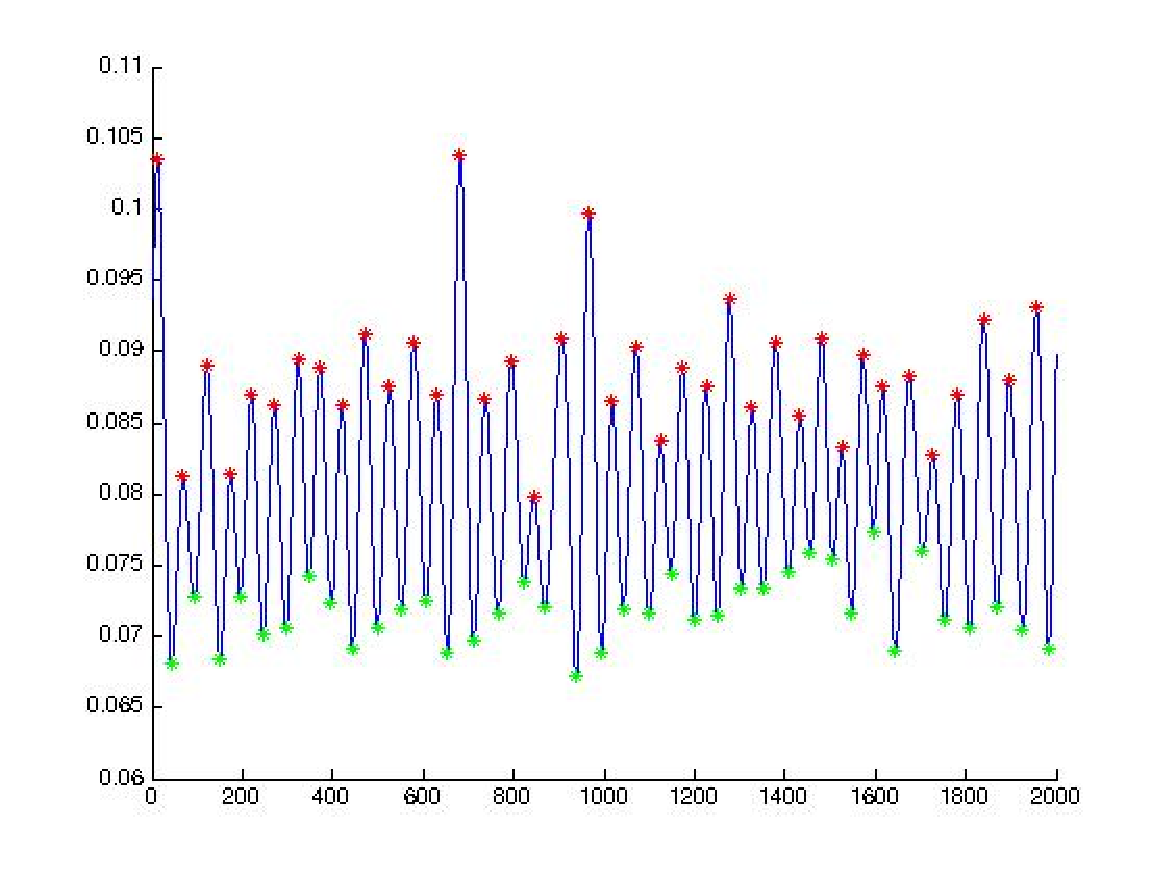
\includegraphics[width=0.36\textwidth]{filtedIM.pdf}
\caption{The clear respiratory MI signal for 2000 frames of volunteer02: the average breathing period is 3.30s and the respiration rate is 18.2 times/minute.}
\label{fig.filteredMI}
\end{figure}

\begin{table}
\newcommand{\tabincell}[2]{\begin{tabular}{@{}#1@{}}#2\end{tabular}}
 \centering
 \begin{tabular}{|c|c|c|c|c|}\hline
 Number & \tabincell{c}{Computational \\Respiratory Rate \\ (times/minute)} & \tabincell{c}{Ground truth\\ (times/minute)} & \tabincell{c}{Time for \\one cycle (s)} \\\hline
V01 & \tabincell{c}{17.1 } & \tabincell{c}{17} & \tabincell{c}{3.51} \\\hline
V02 & \tabincell{c}{18.2} & \tabincell{c}{18} & \tabincell{c}{3.30} \\\hline
V03 & \tabincell{c}{17.3} & \tabincell{c}{17} & \tabincell{c}{3.47} \\\hline
V04 & \tabincell{c}{15.5} & \tabincell{c}{15} &\tabincell{c}{3.87} \\\hline
V05 & \tabincell{c}{15.3} & \tabincell{c}{15} & \tabincell{c}{3.92} \\\hline
V06 & \tabincell{c}{17.8} & \tabincell{c}{18} & \tabincell{c}{3.37} \\\hline
V07 & \tabincell{c}{16.3} & \tabincell{c}{16} & \tabincell{c}{3.75} \\\hline
V08 & \tabincell{c}{17.2} & \tabincell{c}{17} & \tabincell{c}{3.49} \\\hline
V09 & \tabincell{c}{16.3} & \tabincell{c}{16} & \tabincell{c}{3.57}  \\\hline
Real1 & \tabincell{c}{18.2} & \tabincell{c}{18} & \tabincell{c}{3.30}  \\\hline
Real2 & \tabincell{c}{19.2} & \tabincell{c}{19} & \tabincell{c}{3.15}  \\\hline
Real3 & \tabincell{c}{19.3} & \tabincell{c}{19} & \tabincell{c}{3.11}  \\\hline
Real4 & \tabincell{c}{19.8} & \tabincell{c}{20} & \tabincell{c}{3.03}  \\\hline
Real5 & \tabincell{c}{19.0} & \tabincell{c}{19} & \tabincell{c}{3.16}  \\\hline
\end{tabular}
\vspace{0.2 cm}
\caption{Computational results and the ground truth}
\label{tab3.results}
\end{table}
Figure~\ref{fig.breathcycle} is four typical positions of diaphragm. Diaphragm in frame 21 is at its lowest position corresponding to the end of inspiration. Due to the upward diaphragm relaxation during expiration, diaphragm profile in the ultrasound video draws upward and passes through frame 34 until it reaches the end of expiration as shown in frame 46. After expiration ending, the inspiration begins, and diaphragm draws downward due to its contraction and it returns to the original respiratory position in frame 72. This is a typical breathing cycle.
\begin{figure}[h!]
\centering
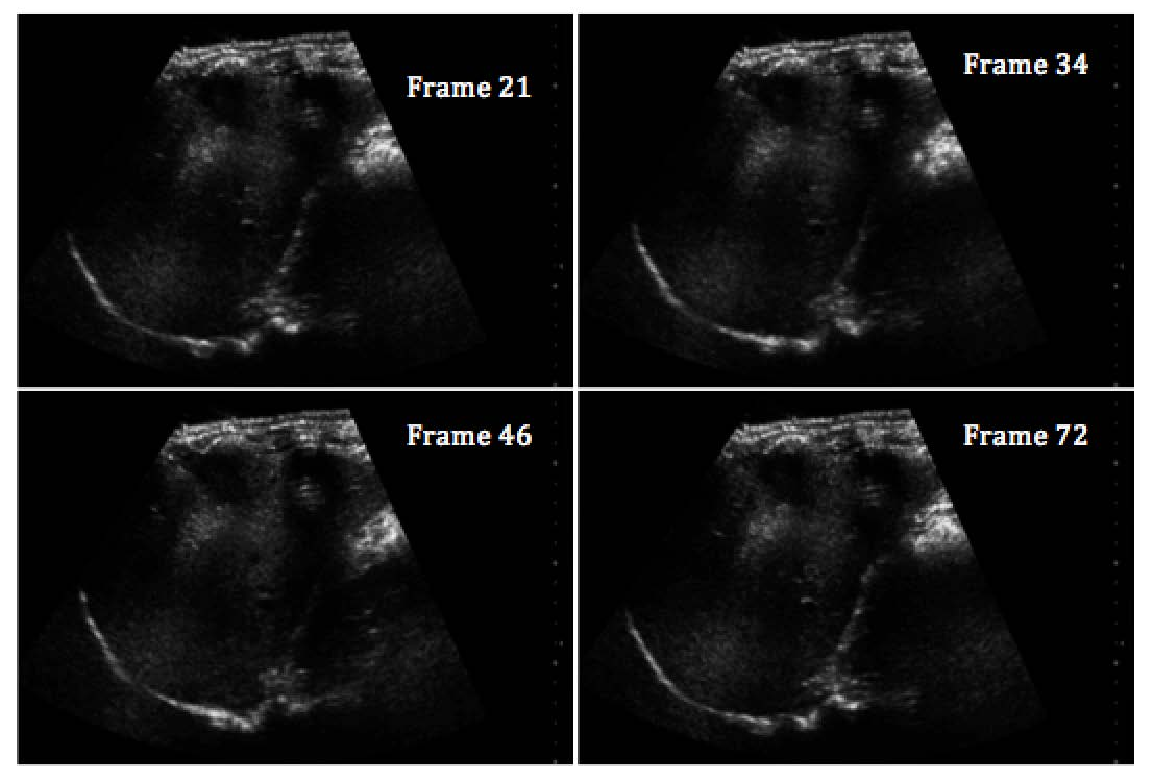
\includegraphics[width=0.36\textwidth]{ucycle.pdf}
\caption{A complete breathing cycle}
\label{fig.breathcycle}
\end{figure}
Figure~\ref{fig.MIcycle} is MI waveform for one respiratory cycle. There are 51 frames in this respiratory cycle. MI value reaches the maximum at frame 1, because this frame is the reference position. As expiration starts, diaphragm draws upward and further away from the reference position. Thus, MI decreases gradually until it reaches to the minimum value at frame 46, the end of expiration. Then diaphragm moves downward and MI increases until it reaches the maximum at the end of inspiration which corresponds to frame 72.
\begin{figure}[h!]
\centering
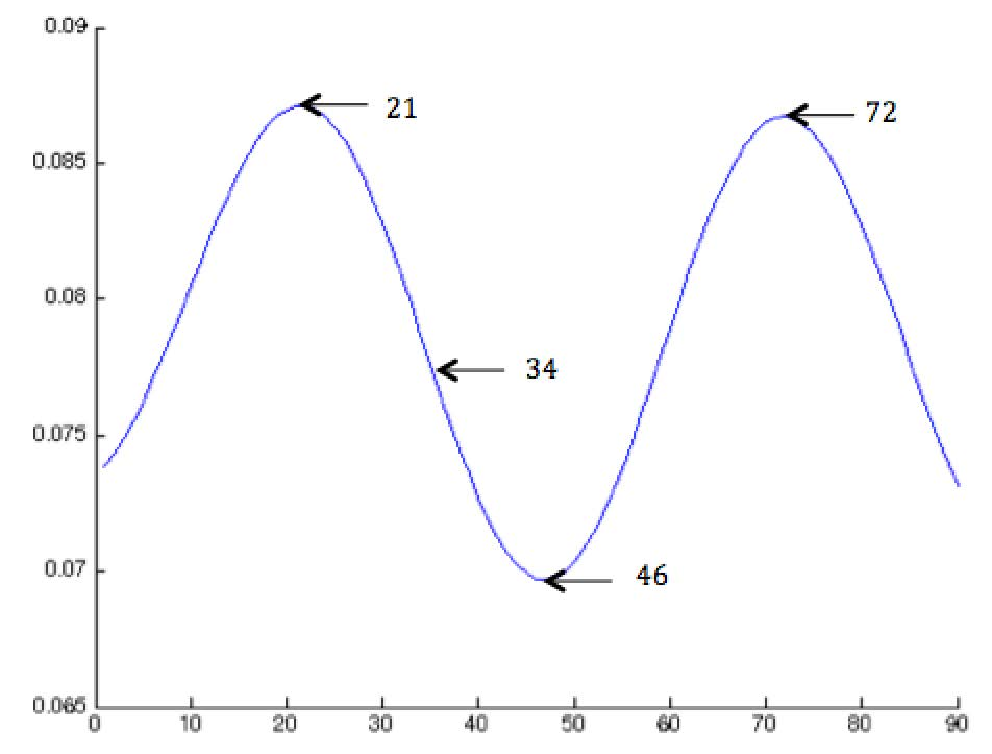
\includegraphics[width=0.36\textwidth]{cycle.pdf}
\caption{Respiratory signal computed by MI method and the corresponding frames. Frames 21 and 72 are captured in the end of inspiration. Frame 46 is captured in the end of expiration.}
\label{fig.MIcycle}
\end{figure}

We also design four templates of respiratory 1D signal, as shown in Figure~\ref{fig.templates}. Pattern of normal breath contains regular cycles and these cycles have same maximum and minimum MI values. Pattern of fast breath has two characteristics: respiration rate is twice faster or more than normal breath and the change of magnitude of each cycle is usually smaller. Apnoea is defined as a complete cessation of oronasal flow for at least 8s; the waveform will be flat for a period of time. Such as the example of apnoea in Figure~\ref{fig.templates}, from frame 100 to frame180, changes of magnitude are negligible. While coughing, subject usually accompanies with several suddenly deep expirations. Therefore, in the pattern of cough, there are obviously peaks which are much higher than other peaks around them. When a subject has asthma attack, irregular breathing activities can be identified from respiratory signals by comparing 1D respiratory waveform with these four templates.
\begin{figure}[h!]
\centering
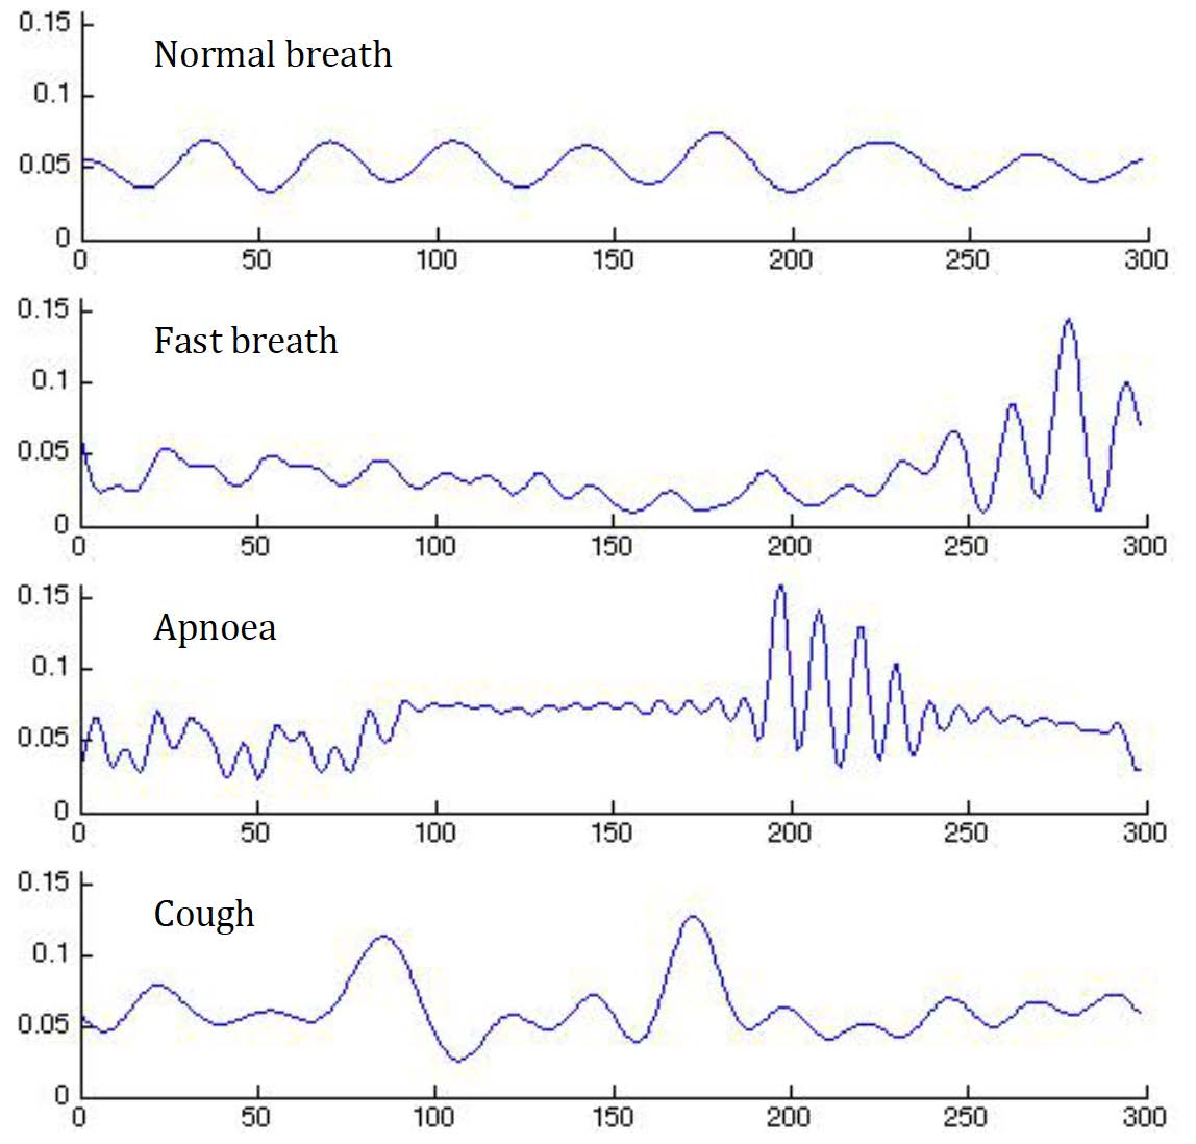
\includegraphics[width=0.36\textwidth]{pattern.pdf}
\caption{Four breathing templates}
\label{fig.templates}
\end{figure}



\section{conclusion and future work} \label{sec.conclusion}
In this paper, an ultrasound monitoring system is proposed for converting 2D image sequence of diaphragm motion to 1D respiratory signal. Four templates of asthma pattern is developed for identifying irregular breathing activities when subject has asthma attack. By using this 2D to 1D method, when the system detects irregular breathing signal, doctors/researchers can retrieve images back to figure out how organ moves at that period. Thus, they can obtain more information of asthmatic analysis. In experiments, the accurate segmentation results ensures the accuracy of MI values and respiration rate estimation. By comparing the computational result with ground truth, the accuracy of the implemented algorithm is verified. Moreover, we explain features of four templates. Based on these features, intervals of a respiratory signal can be classified as one of the four respiratory patterns. In the future, these templates can be used to predict asthma attack. For example, if some patterns occur in specific orders, then the subject is likely to undergo an asthma attack. Because of ultrasound's portability, we can design a portable device for home health monitoring which can extract respiratory signal. Therefore, patients will not need to take asthma exams in hospital periodically. 

\bibliographystyle{abbrv}
\bibliography{sigproc}

\begin{IEEEbiography}
[{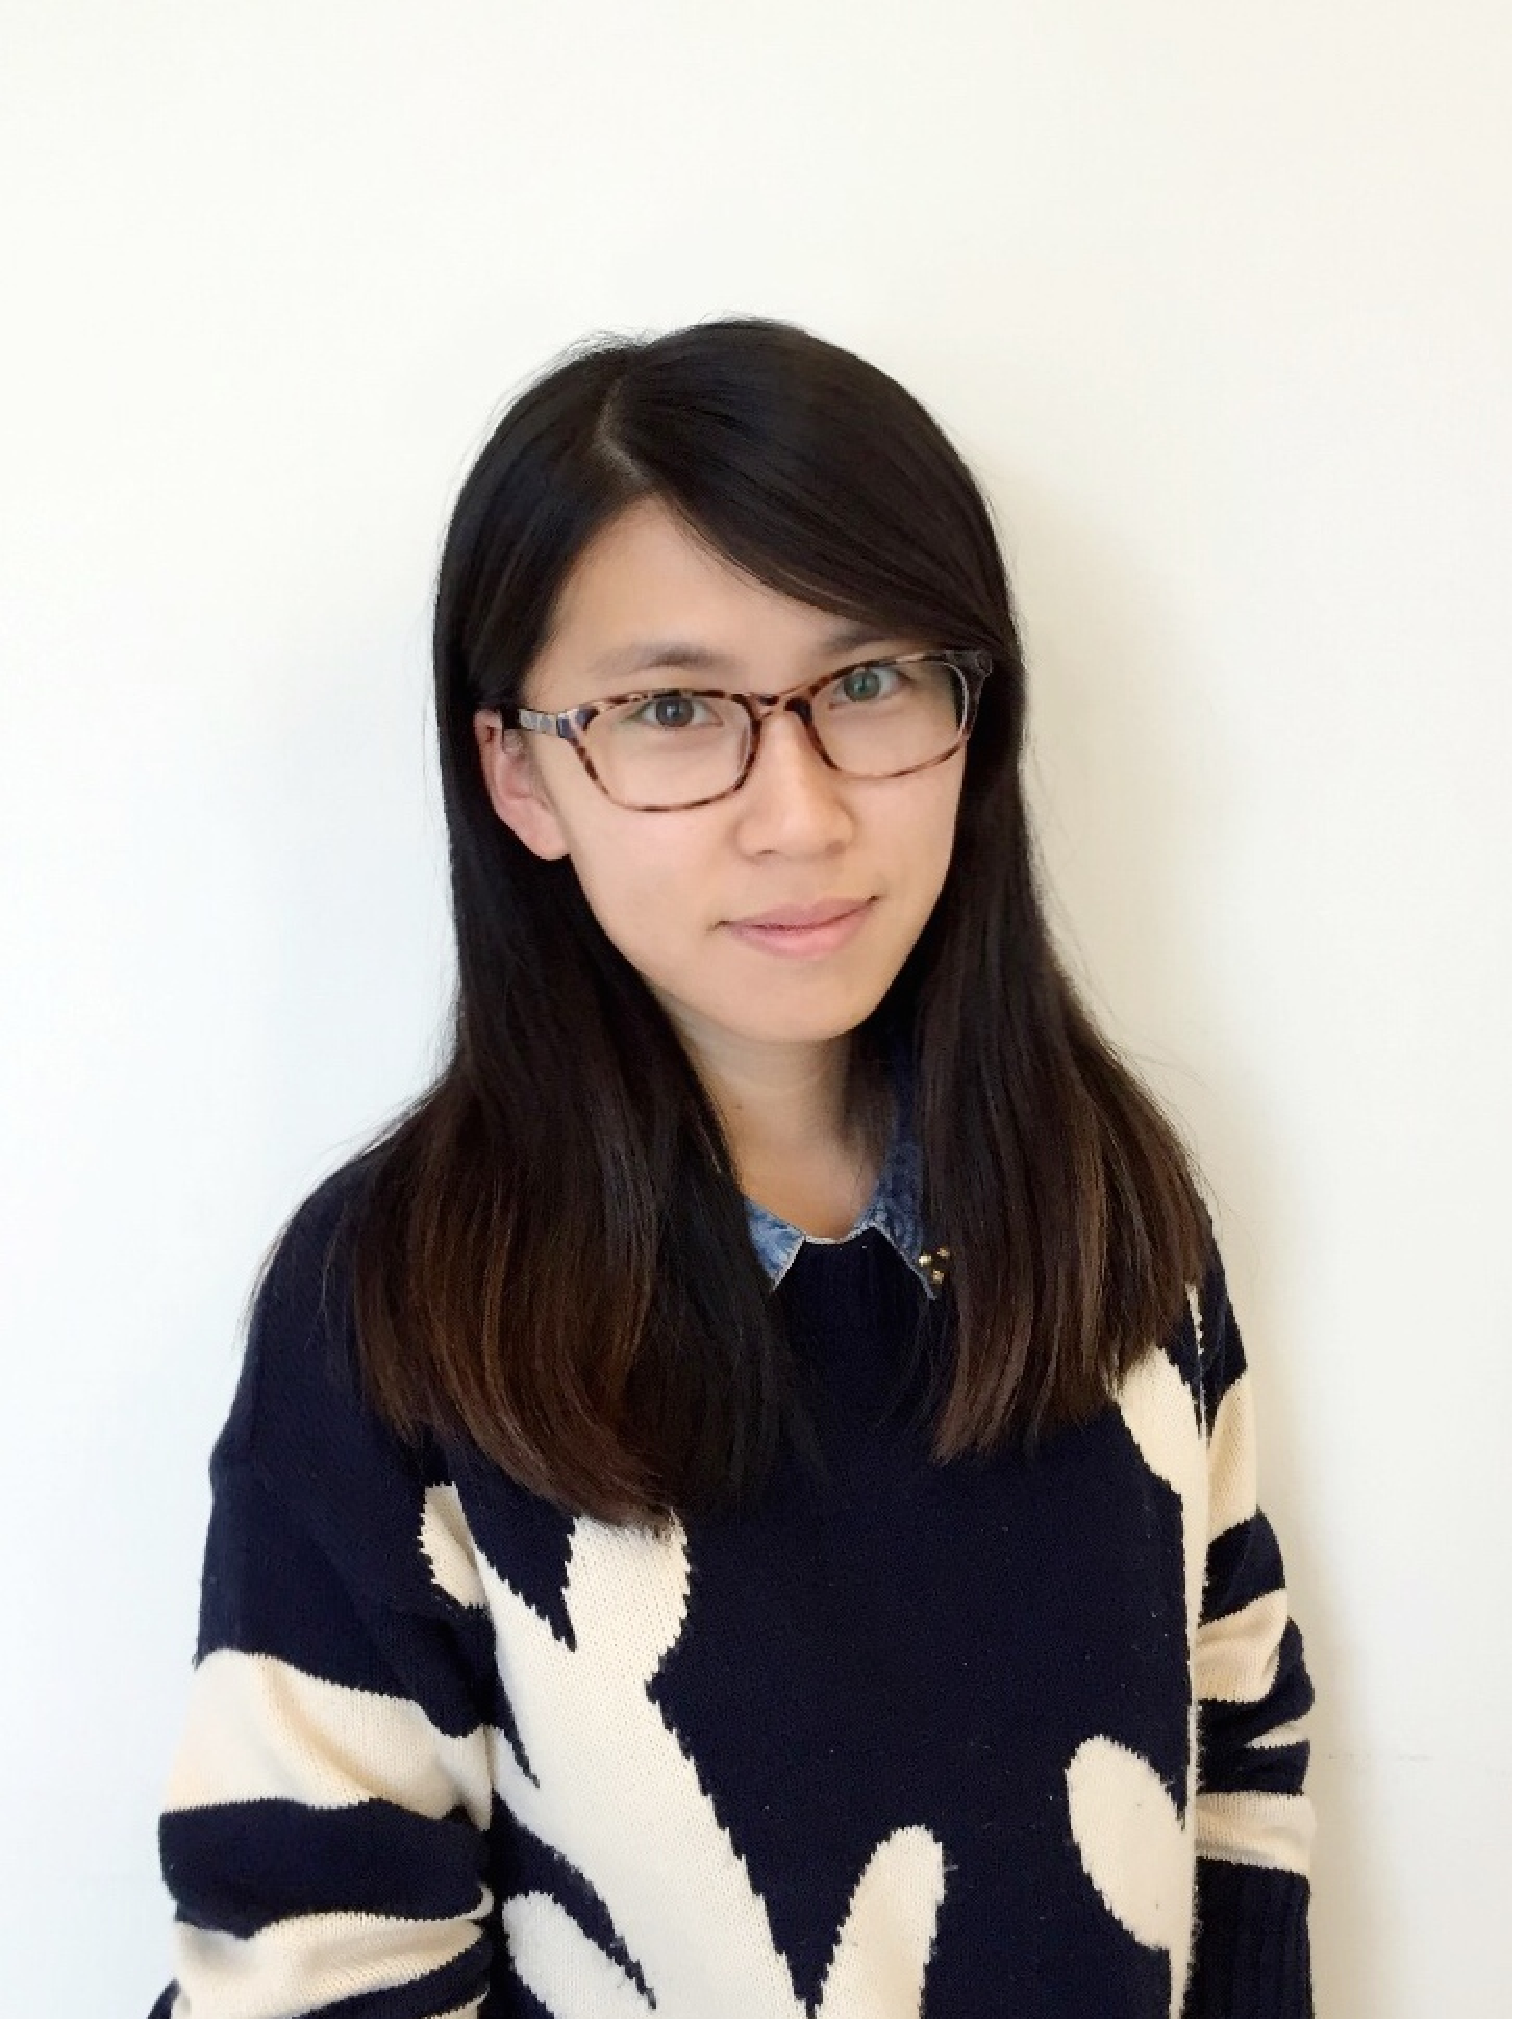
\includegraphics[width=1in,height=1.25in,clip,keepaspectratio]{Liu.pdf}}]
{Menghan Liu} received the B.E. degree in communication engineering from Tianjin University, Tianjin, China. She is currently pursuing the M.S. degree with the Electrical Engineering and Computer Science Department at Case Western Reserve University. Her research interests lie in the area of image processing, computer vision, augmented reality, big data analysis, wearable computing and personal health.
\end{IEEEbiography}
\begin{IEEEbiography}
[{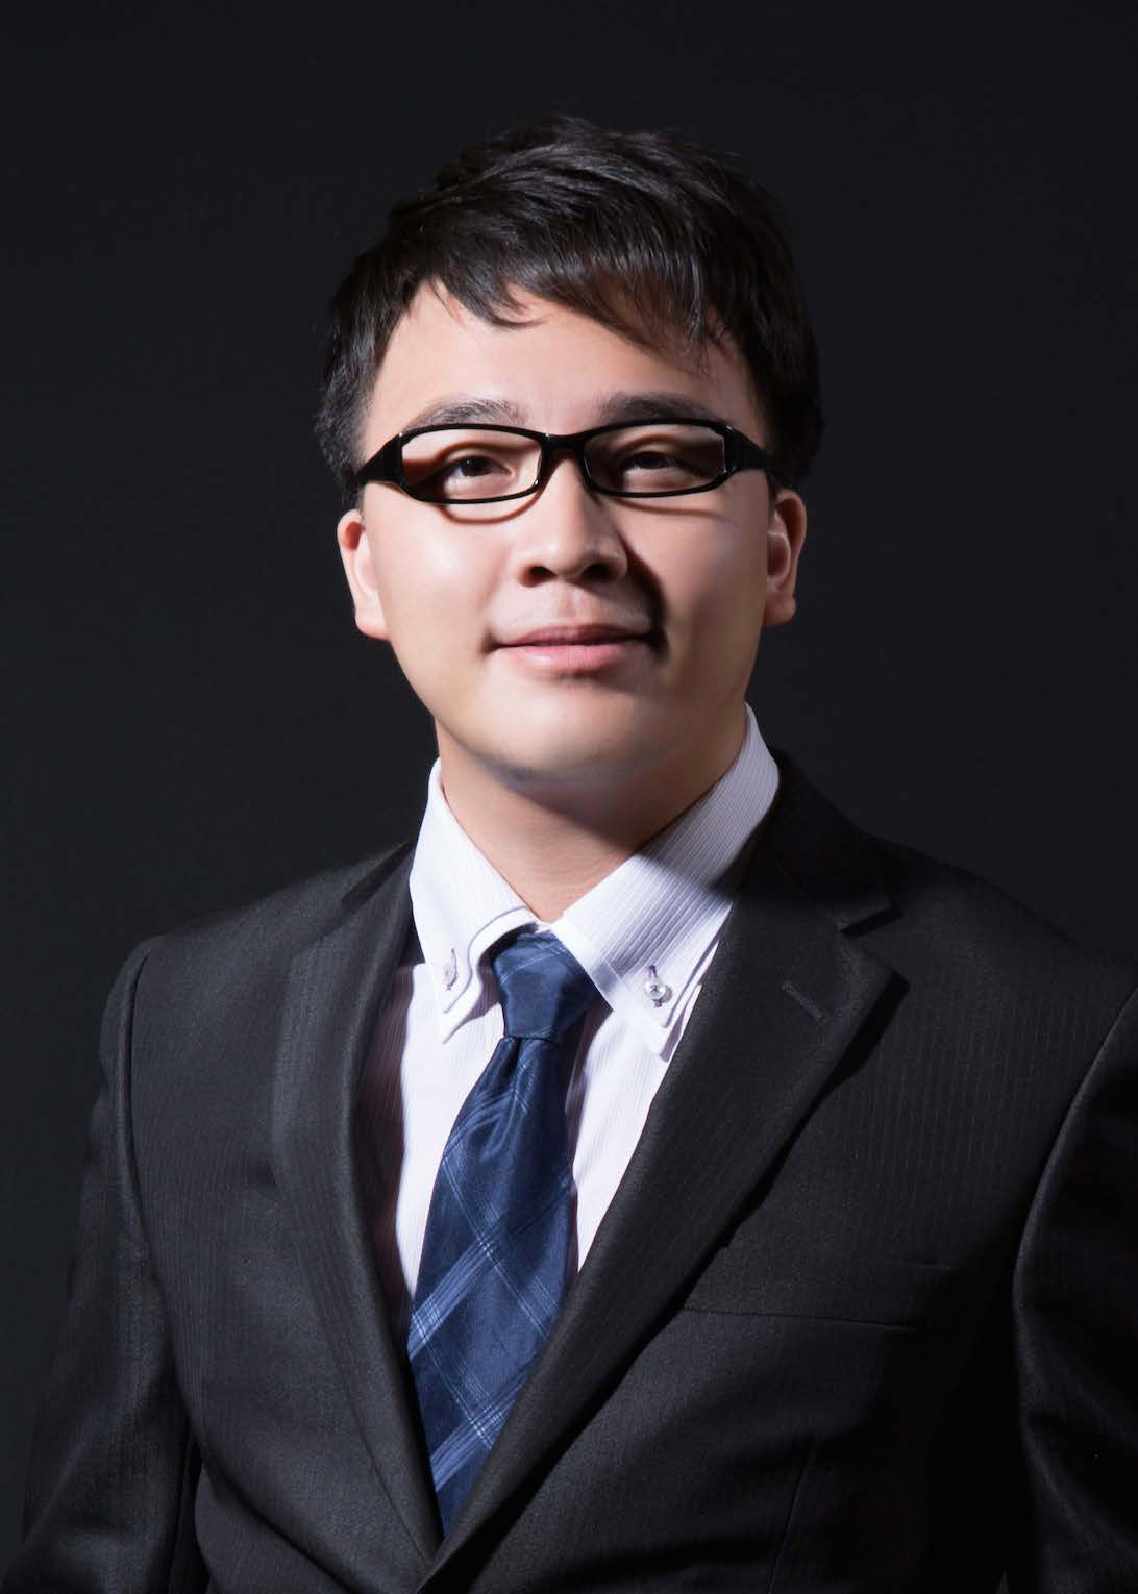
\includegraphics[width=1in,height=1.25in,clip,keepaspectratio]{Huang.pdf}}]
{Ming-Chun Huang} (M'14) is an assistant professor in the Electrical Engineering and Computer Science Department at Case Western Reserve
University~\cite{Sailab}. He has a PhD in computer science from the University of California, Los Angeles (UCLA). Dr. Huang has multiple years
experiences in pressure sensitive medical devices development, pressure map analysis, and physiological signal extraction research.
He is an expert in mHealth, telemedicine, and non-invasive sensing system design. His board research interests includes the area of
wearable computing, health informatics, big data analysis, human computer interaction, sensor, network, augmented reality, and
applications of Internet of Things. He received the Best Medical and Performance Application Paper Award from the IEEE Conference on
Implantable and Wearable Body Sensor Networks in $2013$ and the Best Demonstration Award in ACM Wireless Health Conference in $2011$.
\end{IEEEbiography} 




\end{document}
